\subsection{Multiscale reading of the late research line}
The preceding historical trajectory answers when the candidate-policy regime changed; it cannot resolve a one-thousand-unit gain when the axis spans more than fifteen thousand units. Figure~\ref{fig:late_zoom} therefore uses a separate narrow vertical range. On the Stage 2 bank, the selected checkpoints R8.5 through R9.0 all report area 494,999, while R9.1, R10.0 and the unchanged R10.1 control report 493,965. This is the exact \emph{1,034-unit Stage 2-bank difference}, not the \emph{1,587-unit two-bank difference} of the R9.0--R10.0 paired comparison. The distinction prevents accidental mixing of two aggregation units. These selected archival checkpoints are a development trajectory, not an isolated experiment proving the causal effect of one code edit.
\begin{figure}[htbp]\centering
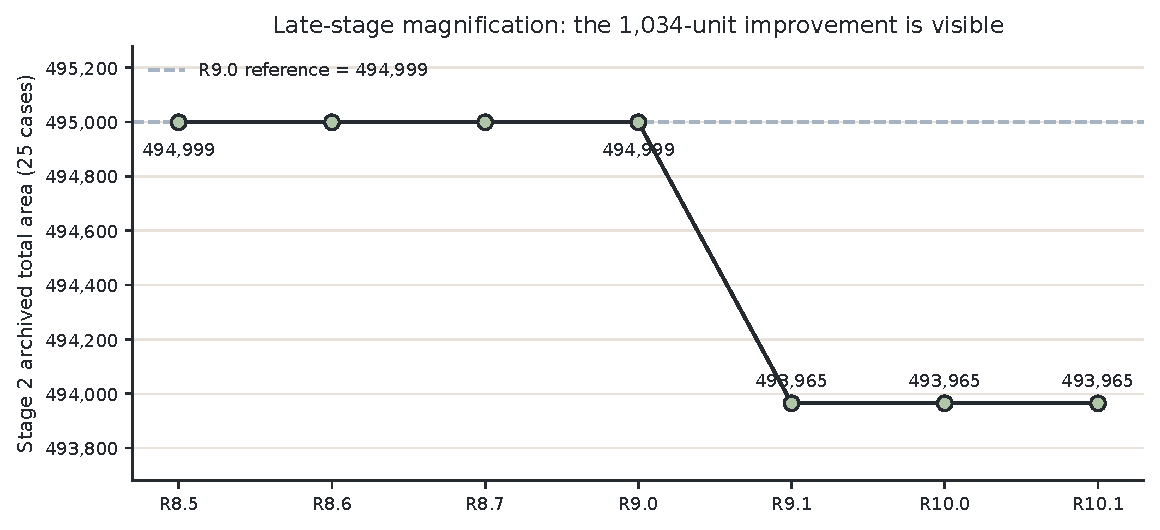
\includegraphics[width=.97\textwidth]{../figures/15_stage2_late_zoom.pdf}
\caption{Late-stage Stage 2 area shown at the resolution needed to see a 1,034-unit change on a roughly 495,000-unit baseline. All points use a complete 25-case checkpoint; cross-version runtime is not inferred from this diagram.}
\label{fig:late_zoom}\end{figure}

\subsection{All 111 named configurations: retain breadth without losing precision}
The experimental inventory contains \textbf{111 distinct (round, variant) names}; \textbf{105} have at least one archived 25-case PASS-and-target-met record, but this does not mean that every repeat of those variants succeeded. The full configuration-by-source listing, including 25-case qualification, observed failures, complete-run minimum/maximum, original report digest, delay, and synthesis runtime, remains in \texttt{data/stage2\_all\_variant\_index.csv}. Rather than presenting eight low-resolution pages of nearly overlapping points, Figure~\ref{fig:variant_spread} asks a more interpretable question: \emph{how much did the alternatives within each Round actually differ?}

The horizontal length is \(\max_v A_v-\min_v A_v\) over qualified archived variants in the same named Round. A symmetric-logarithmic horizontal axis (linear near zero) permits exact zero differences, tens of units, and thousands of units to coexist without making all small differences invisible. The chart thus distinguishes the negligible R7/R7.1/R7.2 variations from broad R8.1--R8.4 exploration, and the more restricted policy changes in R9--R10. It is a \emph{within-Round diversity diagnostic}, not an effect size, confidence interval, or guarantee that the extrema were measured under an interleaved same-executable comparison.
\begin{figure}[htbp]\centering
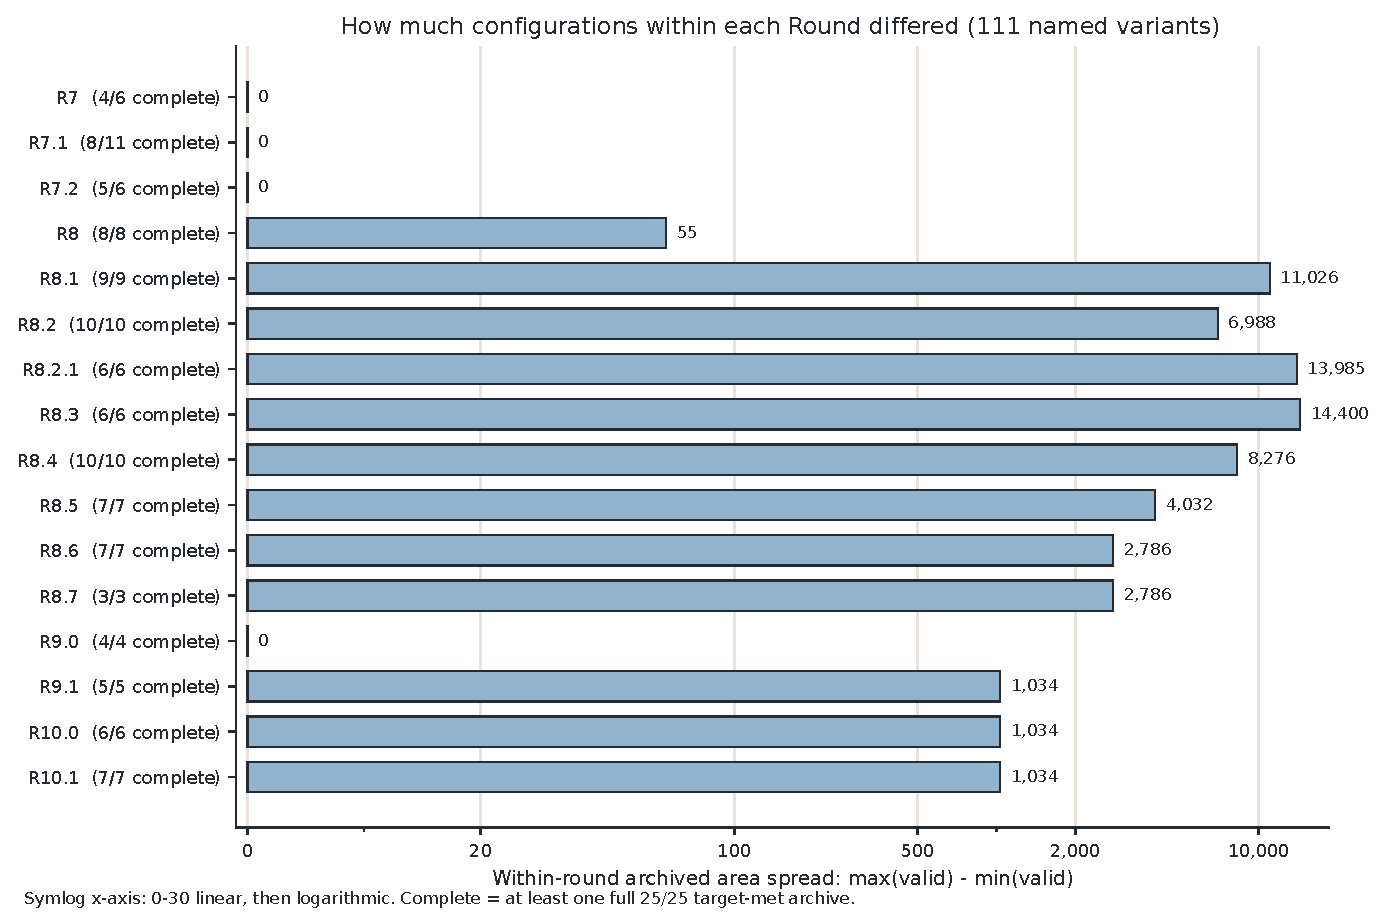
\includegraphics[width=.98\textwidth]{../figures/16_all_variant_spread.pdf}
\caption{Within-Round archived range over complete Stage 2 bank observations, accompanied by qualified/total configuration counts. The horizontal scale uses a linear region near zero and logarithmic growth thereafter; exact original data and evidence paths are preserved in CSV.}
\label{fig:variant_spread}\end{figure}

\subsection{The final policy must be assessed by matched comparison}
The narrow question of whether fewer cut roots or a smaller last-pass budget are preferable \emph{can} be tested on genuinely paired observations. Figure~\ref{fig:archive-finalpolicy} uses 100 matched observations for each R10.1 policy (50 released cases, two repeats). Disabling the final pass yields median runtime ratio \(0.942\) but costs 1,587 weighted area units per 50-case equivalent; caps of 40 and 80 cost 1,008 and 602 units, respectively, while showing only modest median time reductions. A 45-ms allowance costs 241 units and does not improve the observed median runtime (ratio 1.009). Therefore the retained R10.0 policy is a supported \emph{measured operating point}, not a universal optimality theorem or simply the most recent source file.
\begin{figure}[htbp]\centering
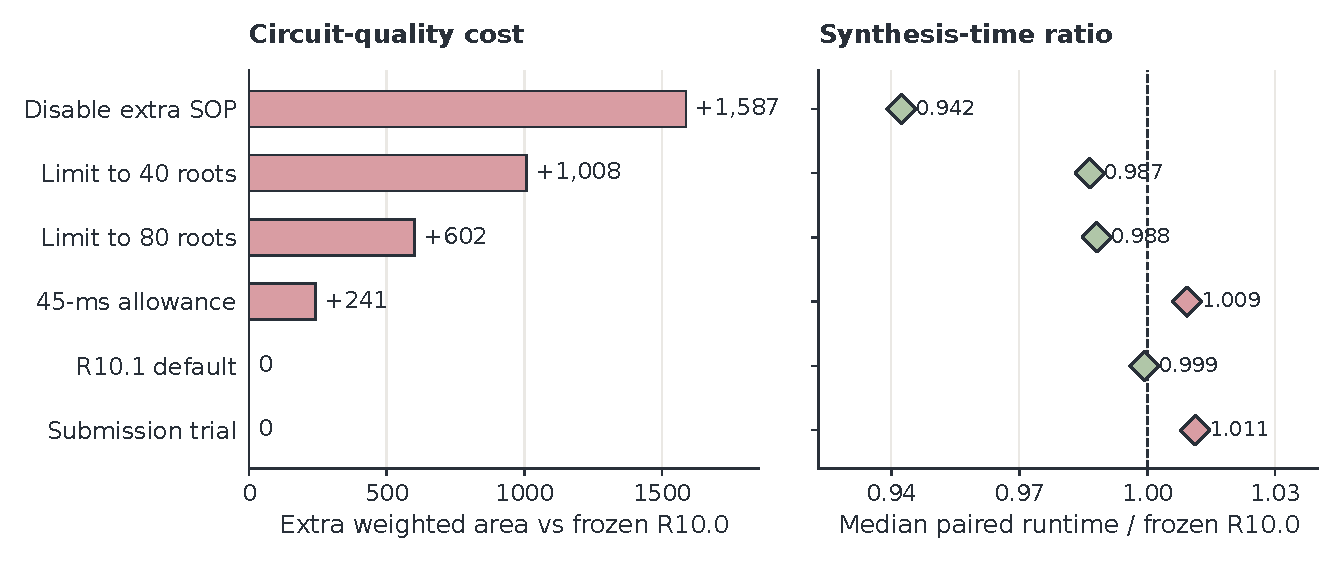
\includegraphics[width=.98\textwidth]{../figures/12_r101_native_pareto.pdf}
\caption{Paired area penalty and synthesis-time ratio relative to frozen R10.0. Positive area penalty is worse; runtime ratios below one are faster. The measurements are converted from 100 paired observations to a 50-case-equivalent area figure.}
\label{fig:archive-finalpolicy}\end{figure}
